
\begin{TP}[Fractale]

\partie{Dans la cour}

Chaque groupe possède une ficelle de 1 mètre de long, une équerre et des craies de couleur.\\[0.5em]
Le but est de reproduire sur le sol de la cour la figure ci‑dessous, constituée de carrés inscrits les uns dans les autres. \\[0.5em]
Le plus grand carré mesure 1 m de côté.\\[0.5em]
Chaque carré a ses sommets positionnés au tiers de la longueur des côtés du carré précédent.\\[0.5em]
Continuez la construction en variant les couleurs pour chaque carré inscrit.\\[0.5em]
\begin{center} 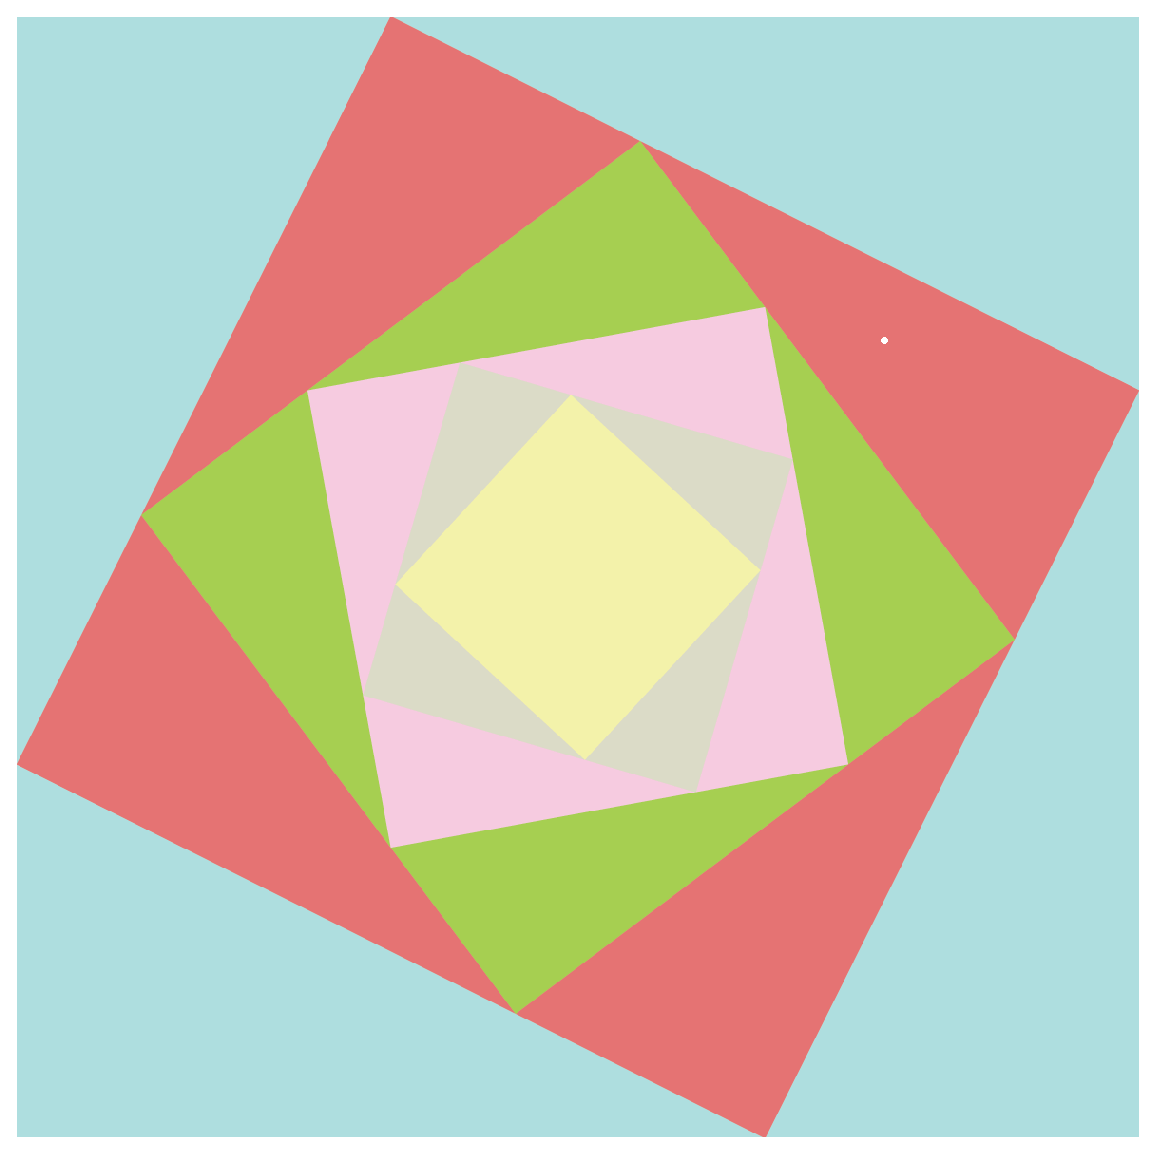
\includegraphics[width=7.4cm]{fractale} \end{center}

\partie{Sur ton cahier}

Sur ton cahier, reproduis la construction de la figure fractale du carré.\\[0.5em]
Selon la même méthode, dessine ensuite une figure fractale d'un losange.

\end{TP}

%%%%%%%%%%%%%%%%%%%%%%%%%%%%%%%%%%%%%%%%%%%%%%%%%%%%%%%%%%%%%%%%

\begin{TP}[Figures téléphonées]

\partie{Construction de la figure}
Chaque élève construit une figure contenant : cinq points, un cercle ayant son rayon ou son diamètre décrit par deux de ces cinq points, un losange. Le reste de la construction est libre.

\partie{Écriture du programme de construction}
Écris un programme de construction de ta propre figure, en indiquant les longueurs utiles et en nommant les points si nécessaire. Donne ensuite ce programme à ton binôme et conserve la figure initiale cachée.

\partie{Reconstruction de la figure}
Essaie de suivre les instructions du programme que tu as reçu et reproduis le plus fidèlement possible la figure de ton camarade.

Une fois les constructions terminées, valide la construction en comparant la figure construite avec l'originale.

\end{TP}

